%archivo_indice.tex
\chapter{Anexos}
	\section{Sistemas operativos}
	El desarrollo del proyecto de memoria tuvo como fin un aplicación para el sistema operativo iOS. Para esto fue necesario utilizar las herramientas dispuestas por Apple Inc.
		\subsection{OSX}
La décima versión del sistema operativo para computadores Macintosh, la X se refiere al numero romano 10. Esta versión posee un micro-núcleo Mach, junto a servicios de sistema operativo de tipo UNIX basados en FreeBSD.
Las aplicaciones para OSX se desarrollan utilizando \textbf{Cocoa} API, la interfaz de programación de aplicaciones orientada a objetos.
%\subsubsection{Xcode}

%		os x, se empezó el desarrollo en lion, migración de xcode 3 a 4, inestabilidad
%		explicar como se usa  itunes con ios
		\subsection{iOS}
Sistema operativo para dispositivos móviles, originalmente fue desarrollado para iPhone, sin embargo se ha utilizado en nuevos productos de Apple como iPod Touch, iPad, y el Apple TV. Su característica principal es la interfaz de usuario basada en manipulación de gestos táctiles por parte del usuario, es decir pellizcos, deslizamientos o toques con los dedos.\\

iOS deriva de Mac OSX en su arquitectura de diseño, utilizando también el mismo micro-núcleo Mach basado en FreeBSD: Darwin.\\

El desarrollo de sus aplicaciones se realiza con \textbf{Cocoa Touch} API (figura \ref{fig:ios-cocoatouch}), la capa de abstracción de iOS.
\begin{figure}[H]
	\centering
	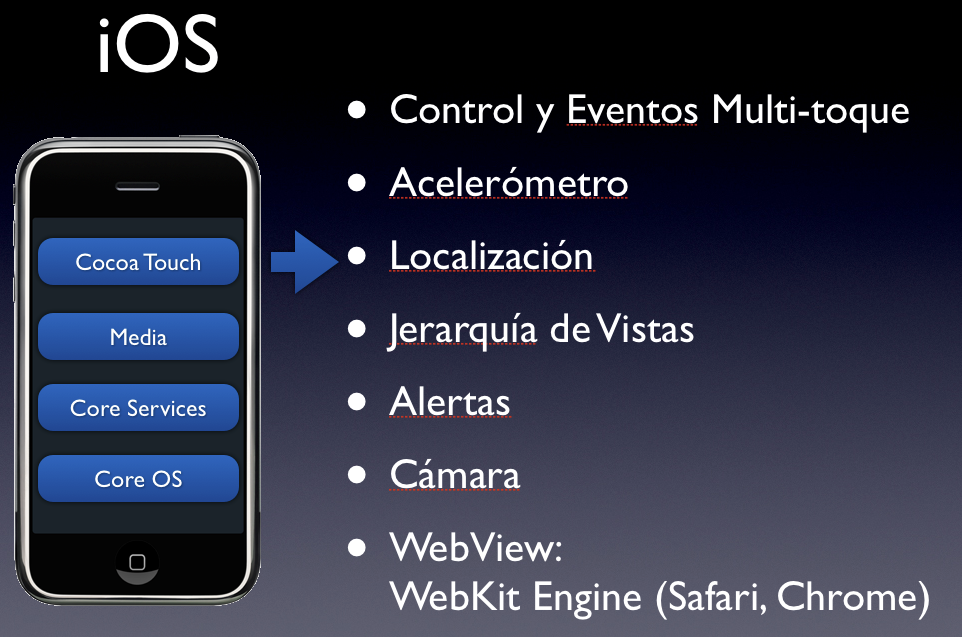
\includegraphics[scale=0.35]{imgs/ios-cocoatouch.png} 
	\caption{Características del dispositivo disponibles a través de Cocoa Touch.}
	\label{fig:ios-cocoatouch}
\end{figure}  

%		se empezó con ios 4, pasamos a 5, luego 6		
%		facilidad de actualizacion

	\section{Hardware}
		%Se presentan los implementos utilizados para desarrollar el proyecto de memoria.
		Este proyecto de memoria tuvo relación con tecnologías y desarrollos de la empresa Apple, razón por la cual se necesitó adquirir dispositivos, tanto por fines de desarrollo como de pruebas.
		\subsection{Macintosh}
		Fue necesario utilizar una computadora Macintosh, debido a la obligación de desarrollar en Xcode y por ende, una computadora que ejecutara el sistema operativo OSX.\\
		
		Los Macintosh, también conocidos simplemente como Mac, son la línea de computadores de escritorio diseñados y manufacturados por Apple Inc. Están enfocados al mercado de computadoras para el hogar, educación y mercado profesional donde además existe la línea \textit{Pro}. Su principal característica es la posibilidad de ejecutar OSX ya que la licencia del sistema operativo sólo permite instalarlo en computadores construidos por Apple Inc \cite{web:license-osx}. Además los Mac que poseen una CPU Intel permiten instalar otros sistemas operativos como Windows y Linux, gracias a la aplicación de OSX \textbf{Bootcamp}.\\
		
		 Una gran diferencia de los Macintosh respecto a un computador de escritorio es en su encendido, ya que partir los Macs utilizan \textbf{EFI} (\textit{Extensible Firmware Interface}) , a diferencia de una computador normal con Windows o Linux que utiliza por defecto la tradicional y retrocompatible \textbf{BIOS} (\textit{Basic Input/Output System}). Esta característica dificulta la instalación de OSX en computadores que no han sido manufacturados por Apple, debido a que parte de sus drivers residen en la partición del disco duro utilizada por la EFI.\\
		 
		 Sin embargo existe el proyecto de \textit{hacking} \textbf{OSx86} \cite{web:osx86} que busca la posibilidad de instalar OSX  en computadores no licenciados. A pesar de existir esta posibilidad, para este proyecto de memoria se utilizó un computador Macbook 7,1 (fig. \ref{img:macbook71}) para evitar cualquier incompatibilidad de software o hardware.
		 
\begin{figure}[H]
	\centering
	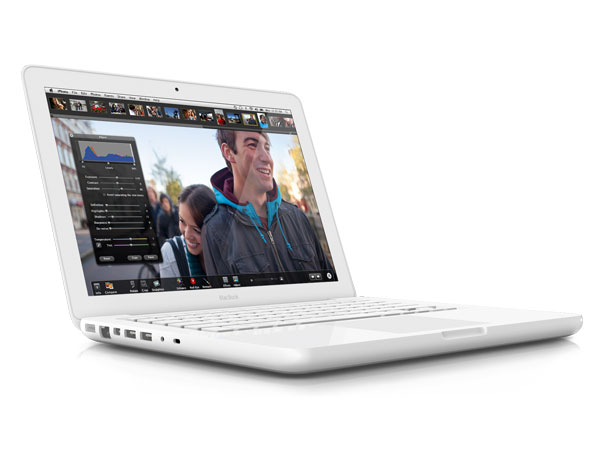
\includegraphics[scale=0.35]{imgs/macbook71.png} 
	\caption{Macbook 7,1. Lanzado al mercado circa 2010.}
	\label{img:macbook71}
\end{figure} 	 
		
%		The Macintosh marketed as Mac, is a line of personal computers (PCs) designed, developed, and marketed by Apple Inc. It is targeted mainly at the home, education, and creative professional markets, and includes the descendants of the original iMac, the entry-level Mac mini desktop model, the Mac Pro tower graphics workstation, and the MacBook Air and MacBook Pro laptops. Its Xserve server was discontinued on January 31, 2011.[2]

%http://en.wikipedia.org/wiki/Unified_Extensible_Firmware_Interface
	
%The use of EFI as opposed to the traditional BIOS. The BIOS found in most PCs is designed for backwards-compatibility to allow the use of older software and operating systems. As Mac OS X has nothing that tied it to the BIOS, it was free to use an alternative firmware that eliminates some of the shortcomings of the BIOS. EFI is not exclusive to Macs, however; motherboards can be purchased off-the-shelf that support EFI, and some computer retailers use it as well now.
%Non-standard motherboard form factors. The motherboards in all current Macintosh models do not correspond to a form factor found in other retailer's computers, such as ATX or ITX.
%Unique case deigns. Macintosh cases are designed to be slightly more "classy" looking than those found with the standard "white box" PC.
%Incompatible expansion cards. Because of the aforementioned use of EFI, off-the-shelf expansion cards such as graphics cards cannot be used in a Mac. Similar models designed for use with EFI can be purchased from the Apple store, at a typically higher markup price. This,too, will probably change as EFI becomes more widespread.

		\subsection{iPhone, iPad, iPod Touch}
		
El \textbf{iPhone} (fig. \ref{sshot_iOS_sstream}), es el smartphone creado por Apple en 2007. Este producto revolucionó el mercado de la telefonía móvil al popularizar las pantallas táctiles y el enlace a Internet a través de las redes celulares. \\

El desarrollo de este dispositivo data desde 2004 gracias a la investigación por parte de Apple Inc. de pantallas capacitivas para lograr gesto multitáctiles. Originalmente este desarrollo correspondía a la idea de un dispositivo táctil que asemeje el uso del papel real en pantallas del tamaño de un folio, lo que posteriormente se manifestaría en forma del \textbf{iPad} (fig. \ref{img:ipad-hw}), y por consiguiente un nuevo mercado: computadores \textbf{Tablet}.\\

Para ampliar el mercado del sistema operativo iOS, Apple también reformuló su ya popular reproductor de multimedia iPod para dar paso al \textbf{iPod Touch}, el cual no difiere mucho de un iPhone sin tomar en cuenta la conectividad a las redes celulares para realizar llamadas y mantener una conexión persistente a Internet.\\

En materia de software estos tres dispositivos tienen en común la ejecución de \textbf{iOS} como sistema operativo, sin embargo respecto al hardware, iPad destaca por disponer de una pantalla táctil de 10 pulgadas (diagonales) de tamaño, lo cual significa distintas prestaciones de las aplicaciones para el usuario. Sin embargo iPad permite la ejecución de aplicaciones desarrolladas exclusivamente para modelos de pantalla pequeña (4 pulgadas diagonales) con un modo de escalado, como lo fue con la aplicación desarrollada en este proyecto.

\begin{figure}[H]
	\centering
	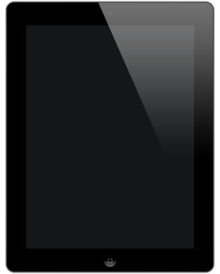
\includegraphics[scale=0.4]{imgs/ipad-hw.png} 
	\caption{iPad, lanzado al mercado el 3 de Abril de 2010.}
	\label{img:ipad-hw}
\end{figure} 	 
		 
	\section{Software}
Apple pone a disposición de los desarrolladores de aplicaciones para sus productos, una gran cantidad de software accesible desde el sitio web \textit{Downloads for Apple Developers} \cite{apple-repositorio}.
		\subsection{Xcode}
		\label{anexo:xcode}
		Para este proyecto se utilizó el entorno de desarrollo \textbf{Xcode}, el cual está solamente disponible para OSX.\\

Xcode se puede obtener, además del repositorio para desarrolladores \cite{apple-repositorio}, desde la tienda de aplicaciones de OSX, el repositorio que integra el mismo sistema de pago utilizado en la tienda de música digital iTunes Store (figura \ref{fig:xcode-appstore}).
\begin{figure}[H]
	\centering
	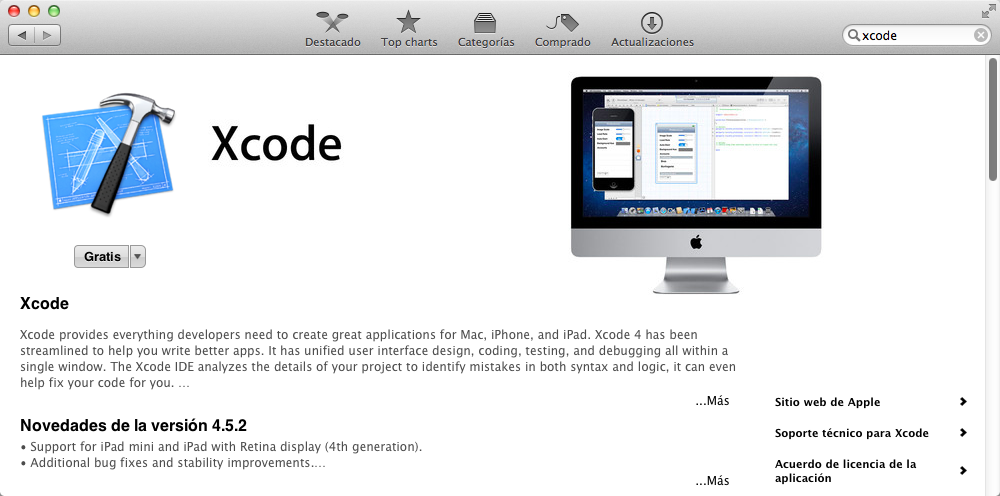
\includegraphics[scale=0.4]{imgs/xcode-appstore.png} 
	\caption{Xcode disponible gratis en la Mac App Store, la tienda de aplicaciones para OSX}
	\label{fig:xcode-appstore}
\end{figure}  

		\subsection{Configuración de Xcode para depuración de scheme}
		\label{anexo:xcode-debug}
		Este ajuste se logra editando el esquema (\textit{scheme}) de la compilación, no confundir con el esquema (\textit{scheme}) del URL. El entorno de desarrollo Xcode permite administrar distintos esquemas de compilación, siendo \textit{Build}, \textit{Run}, \textit{Analyze} y \textit{Archive} los más utilizados. Para mantener Xcode atento al lanzamiento de la compilación se debe editar el esquema \textbf{\textit{Run}} (ejecutar) como se muestra en la figura \ref{fig:xcode-debug-wait}.
  
%	- clientes de twitter en iPhone, twitter y Tweetbot, debug en el método e imprimir en consola la app que lo lanzó.  
%	- debug con app en background
%	- debug con app cerrada y a la espera que parta por otra aplicación
%	explicar que se detuvo la carga del stream cuando está cerrada y que se espera una notificacion de la carga de la UI antes de cargar el stream.
    
\begin{figure}[H]
	\centering
	\begin{tabular}{cc}
	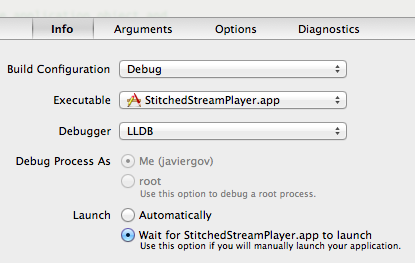
\includegraphics[scale=0.7]{imgs/xcode-debug-wait.png}
	\end{tabular}
	\caption{Configuración de Xcode para pruebas de lanzamiento de la aplicación por scheme.}
	\label{fig:xcode-debug-wait}
\end{figure}

%		descripcion de iphone, cuando salió, presentación de steve, revolucion del smartphone, pasar de teclas a nuevas pantallas táctiles.
%		ipad, nueva forma de leer, reemplaza netbook, 3g pero no llama, creó un nuevo mercado y es lider
%		ipod, comezó como música, luego de iphone adopta ios, explicar que es alternativa a iphone, gran adopcion en usa.  lider en players.


%	\section{Frameworks}
%	uikit, descripción 
%	avfoundation, descripcion
%	mpmedia framework, descripcion
	%entorno de desarrollo utilizado
	
%\chapter{Bibliografia}
	% refencias de lo estudiado y utilizado para el trabajo